\documentclass[oneside,a4paper,10pts,article]{memoir}
\usepackage[utf8]{inputenc}

\usepackage[danish]{isodate}

\usepackage{palatino}
\usepackage{graphicx}
\usepackage{todonotes}
\presetkeys{todonotes}{inline}{}

\usepackage{url}
\usepackage[hidelinks,hyperindex]{hyperref}

\captionnamefont{\bfseries}

\usepackage{tikz}
\usetikzlibrary{positioning,arrows,calc}

\newcommand{\vs}{%
    \tikz[remember picture,overlay]{\node at
        ($(current page.south east)+(-2,2)$)
        [anchor=south east] {Vend siden $\rightarrow$};}
}

\usepackage{listings}
\lstdefinelanguage{JavaScript}{
  keywords={break, case, catch, continue, debugger, default, delete,
    do, else, false, finally, for, function, if, in, instanceof, new,
    null, return, switch, this, throw, true, try, typeof, var, void,
    while, with},
  morecomment=[l]{//},
  morecomment=[s]{/*}{*/},
  morestring=[b]',
  morestring=[b]",
  ndkeywords={class, export, boolean, throw, implements, import, this},
  keywordstyle=\color{blue},
  ndkeywordstyle=\color{darkgray},
  identifierstyle=\color{black},
  commentstyle=\color{purple}\ttfamily,
  stringstyle=\color{red}\ttfamily,
  sensitive=true,
  extendedchars=true,
literate=%
{æ}{{\ae}}1
{å}{{\aa}}1
{ø}{{\o}}1
{Æ}{{\AE}}1
{Å}{{\AA}}1
{Ø}{{\O}}1
}

\lstset{
  basicstyle=\ttfamily\footnotesize,
  keywordstyle=\bfseries,
  captionpos=b,
  language=JavaScript
}

% Remove section numbers
\setsecnumdepth{part}

% Remove page numbers
\renewcommand\thepage{}

\title{Funktioner i Processing
  \\ {\normalfont\small\scshape Coding Pirates DIKU }} \date{\today}

\begin{document}
\maketitle
\vs
\vspace{-10mm}
\chapter{Funktioner}
En fiske-funktion:
\begin{lstlisting}
var fish = function (xpos, ypos) {
    ellipse(xpos, ypos, 120, 75);
    triangle(xpos-60, ypos, xpos-90, ypos-30, xpos-90, ypos+30);
};
    
fish(100);
fish(300);
\end{lstlisting}
\vspace{-3mm}
\chapter{Tilfældige fisk}
\begin{lstlisting}
draw = function () {
    var x = random(0, width);
    var y = random(0, height);
    fish(x, y);
};
\end{lstlisting}
\vspace{-3mm}
\chapter{Opgaver}
\begin{itemize}
\item Vælg tilfældige farver på fiskene.
\item Skriv en \texttt{ufo(x,y)}-funktion.
\item Tegn en Pokéball (eller noget andet) og gør det til en funktion.
\item Tegn dine Pokéball's i tilfældige størrelser, tilfældige steder.
\end{itemize}

\hspace{-20mm}
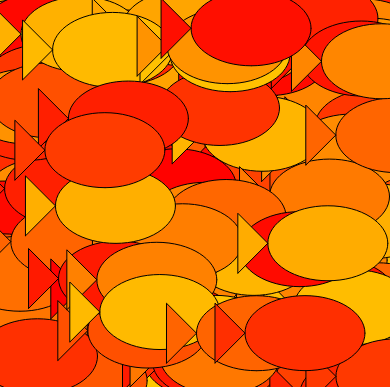
\includegraphics[width=0.4\textwidth]{pics/flerefisk.png}
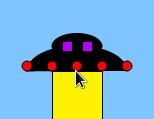
\includegraphics[width=0.2\textwidth]{pics/ufo.png}

\includegraphics[width=0.2\textwidth]{pics/pokeball.png}
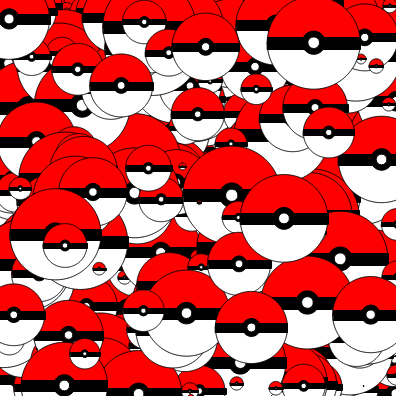
\includegraphics[width=0.4\textwidth]{pics/pokeballs.png}


\newpage
\chapter{UFO-spil}
\begin{lstlisting}
var ufoX = 200;
var hastighedX = 0;

keyPressed = function () {
  if (keyCode === LEFT) {
    hastighedX = -5;
  }
  if (keyCode === RIGHT) {
    hastighedX = 5;
  }
}

draw = function () {
   background(255,255,255);
   ufo(ufoX, mouseY);
   ufoX = ufoX + hastighedX;
}
\end{lstlisting}

\chapter{Opgaver}
\begin{itemize}
\item Lav en \texttt{ufoY} variabel.
\item Lav en \texttt{hastighedY} variabel.
\item Gør så piletasterne op/ned ændrer \texttt{hastighedY} variablen ($\pm5$).
\item Gør så \texttt{ufoY} variablen ændres i forhold til hastigheden.
\end{itemize}

\chapter{UFO laserkanon}
\begin{lstlisting}
  if(mouseIsPressed===true){
    line(ufoX, ufoY, mouseX, mouseY);
  }
\end{lstlisting}

\chapter{Opgaver}
\begin{itemize}
\item Gør laser-kanonen kraftigere med \texttt{strokeWeight(<bredde>)}
\item Få laseren til at blinke i forskellige farver!
\end{itemize}

\hspace{1cm}
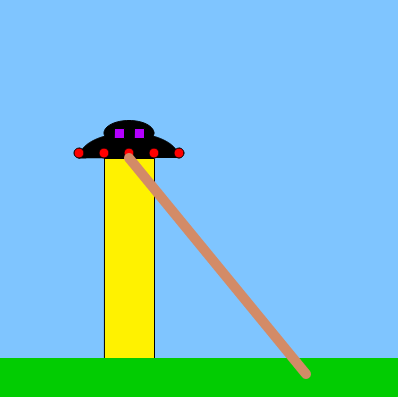
\includegraphics[width=0.4\textwidth]{pics/laserkanon.png}

\end{document}